\documentclass[a4paper]{article}
%% Language and font encodings
\usepackage[english]{babel}
\usepackage[utf8x]{inputenc}
\usepackage[T1]{fontenc}

%% Sets page size and margins
\usepackage[a4paper,top=3cm,bottom=2cm,left=3cm,right=3cm,marginparwidth=1.75cm]{geometry}

%% Useful packages
\usepackage{amsmath}
\usepackage{amssymb}
\usepackage{graphicx}

\usepackage{algorithm} 
\usepackage{algpseudocode} 


% For multiple pages in a pdf document
\usepackage{pdfpages}

\usepackage{listings}
\usepackage{color} %red, green, blue, yellow, cyan, magenta, black, white
\definecolor{mygreen}{RGB}{28,172,0} % color values Red, Green, Blue
\definecolor{mylilas}{RGB}{170,55,241}

\lstset{language=Matlab,%
    %basicstyle=\color{red},
    breaklines=true,%
    morekeywords={matlab2tikz},
    keywordstyle=\color{blue},%
    morekeywords=[2]{1}, keywordstyle=[2]{\color{black}},
    identifierstyle=\color{black},%
    stringstyle=\color{mylilas},
    commentstyle=\color{mygreen},%
    showstringspaces=false,%without this there will be a symbol in the places where there is a space
    numbers=left,%
    numberstyle={\tiny \color{black}},% size of the numbers
    numbersep=9pt, % this defines how far the numbers are from the text
    emph=[1]{for,end,break},emphstyle=[1]\color{red}, %some words to emphasise
    %emph=[2]{word1,word2}, emphstyle=[2]{style},    
}
\title{AEROSP 588 Homework 1}
\author{Andi Zhou}
\begin{document}
\maketitle

\section{Question 1}
We are given the following one-dimensional function:
\begin{equation}
    f(x) = \frac{1}{12} x^4 + x^3 -16x^2 + 4x + 12
\end{equation}
We are asked to plot the function, and find and classify the minimum graphically. Using \texttt{Python} and \texttt{matplotlib}, we obtain the following plot (Figure \ref{fig:Q1_F1}):
\begin{figure}[h]
    \centering
    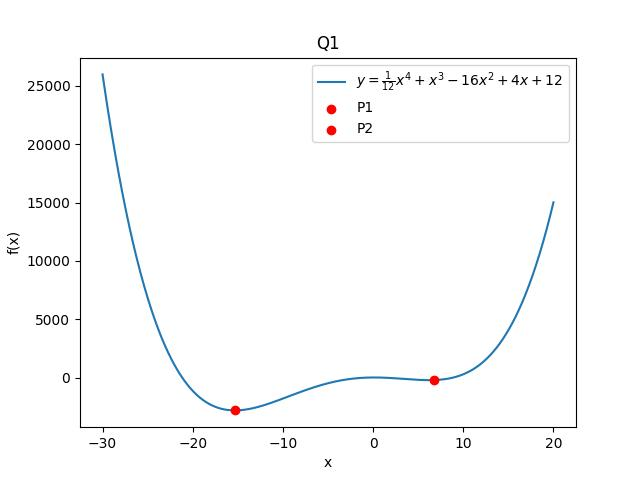
\includegraphics[width = 8cm]{HW1/Picture/Q1_F1.jpeg}
    \caption{Plotted $f(x)$}
    \label{fig:Q1_F1}
\end{figure}
Where with the red dots, we have identified graphically one global minimum (left) and one local minimum (right). Local minimum is classified as a point that is better than any other point within a small neighborhood, which the right point clearly suffice. As for left point, we classify it as a global minimum since this is the lowest point within the entire function. We could invesitigate this graphically by expanding the function domain (Figure \ref{fig:Q1_F2}):
\begin{figure}[H]
    \centering
    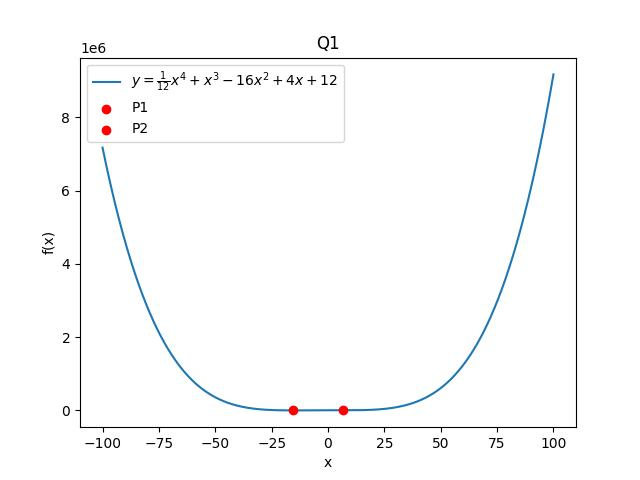
\includegraphics[width = 8cm]{HW1/Picture/Q1_F2.jpeg}
    \caption{Zoomed out plot for Q1}
    \label{fig:Q1_F2}
\end{figure}
We see that as the plot zooms out, the bounds continues to increase indefinitely. Therefore, we have two minimums within this function.

\section{Question 2}

\end{document}
